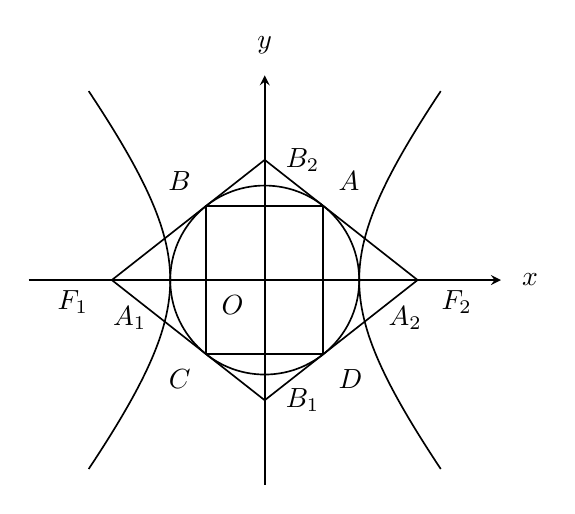
\begin{tikzpicture}[x=1cm,y=1cm,line width=.6pt]
% e=(1+sqrt5)/2; a=1.2,b=1.526423579417,c=1.942; tangent rectangle from foot of perpendicular
\coordinate (O) at (0,0);
\coordinate (F1) at (-1.9416407865,0.0000000000);
\coordinate (F2) at (1.9416407865,0.0000000000);
\coordinate (A1) at (-1.2,0);
\coordinate (A2) at (1.2,0);
\coordinate (B1) at (0.0000000000,-1.5264235794174235794);
\coordinate (B2) at (0.0000000000,1.5264235794174235794);
\coordinate (RA) at (0.7416407865,0.9433816533);
\coordinate (RB) at (-0.7416407865,0.9433816533);
\coordinate (RC) at (-0.7416407865,-0.9433816533);
\coordinate (RD) at (0.7416407865,-0.9433816533);
\draw[-stealth] (-3,0)--(3,0) node[right,xshift=4pt] {$x$};
\draw[-stealth] (0,-2.6)--(0,2.6) node[above,yshift=4pt] {$y$};
% hyperbola branches: x=a*sqrt(1+(y/b)^2)
\draw[domain=-2.4:2.4,samples=60,smooth] plot ({1.2*sqrt(1+(\x/1.526423579417)^2)},\x);
\draw[domain=-2.4:2.4,samples=60,smooth] plot ({-1.2*sqrt(1+(\x/1.526423579417)^2)},\x);
% circle radius a
\draw (0,0) circle (1.2);
% rhombus F1-B2-F2-B1
\draw (F1)--(B2)--(F2)--(B1)--cycle;
% tangent rectangle
\draw (RA)--(RB)--(RC)--(RD)--cycle;
\node[below left,xshift=-4pt,yshift=-2pt] at (O) {$O$};
\node[below left,xshift=-5pt] at (F1) {$F_{1}$};
\node[below right,xshift=5pt] at (F2) {$F_{2}$};
\node[below left,xshift=-5pt,yshift=-6pt] at (A1) {$A_{1}$};
\node[below right,xshift=7pt,yshift=-6pt] at (A2) {$A_{2}$};
\node[right,xshift=4pt] at (B2) {$B_{2}$};
\node[right,xshift=4pt] at (B1) {$B_{1}$};
\node[above right,xshift=2pt,yshift=2pt] at (RA) {$A$};
\node[above left,xshift=-2pt,yshift=2pt] at (RB) {$B$};
\node[below left,xshift=-2pt,yshift=-2pt] at (RC) {$C$};
\node[below right,xshift=2pt,yshift=-2pt] at (RD) {$D$};
\end{tikzpicture}
